\documentclass[a4paper,11pt]{article}
\usepackage[cmex10]{amsmath}
\usepackage{amsfonts,amssymb}
\usepackage{amsthm}
\usepackage{IEEEtrantools}
\usepackage[usenames,dvipsnames]{color}
\usepackage{colortbl}
\usepackage{framed}
\usepackage[pdftex]{graphicx}
\graphicspath{{../pdf/}{../jpeg/}{../png/}}
\DeclareGraphicsExtensions{.pdf,.jpeg,.png}
\usepackage[margin=1.5in]{geometry}
\usepackage{enumerate}
\usepackage{bm}
\usepackage{float,url}
\usepackage{array,changepage}
%\usepackage{epstopdf}




\begin{document}
\title{Exercise 1}
\author{Bowen Hua}
\date{\today}
\maketitle

\section{Linear Regression}
\subsection{(A)}
Matrix form:
$$
\hat{\beta} = \arg \min_{\beta \in \mathcal{R}^P} \frac{1}{2} (y - X \beta)^T W(y - X \beta).
$$

Since $W$ is symmetric and positive semidefinite, this is a convex optimization problem. Its first-order optimality condition is necessary and sufficient:
$$
X^TW(y - X\beta) = \bm{0}.
$$
\subsection{(B)}

\subsubsection{Method 1: direct inversion}

Described in the problem statement:
$$
\beta = (X^T W X)^{-1} X^T W y.
 $$

To exploit sparsity of $W$, we use broadcasting in Python instead of matrix multiplication to compute operations w.r.t.\ $W$ matrix. This method has a complexity of $O(np^2)$.
\subsubsection{Method 2: pseudoinverse}

Since the weight matrix $W$ is diagonal, we can define ${W}^{\frac{1}{2}}$ to be a diagonal matrix where the $i$-th diagonal element equals $\sqrt{w_i}$. Now we can re-write the optimality condition:
$$
\beta  = [({W}^{\frac{1}{2}}X)^T  ({W}^{\frac{1}{2}}X)]^{-1}  ({W}^{\frac{1}{2}}X)^T y,
$$
which we re-write as
$$
\beta  = ({W}^{\frac{1}{2}}X)^\dagger {W}^{\frac{1}{2}} y,
$$
where $({W}^{\frac{1}{2}}X)^\dagger$ is the pseudoinverse of ${W}^{\frac{1}{2}}X$.

We first ``preprocess'' the feature matrix $X$ and $y$ by multiplying ${W}^{\frac{1}{2}}$ on the left. 

We then compute the pseudoinverse through computing SVD of ${W}^{\frac{1}{2}}X$. This method is numerically more stable than the direct inverse method. (There could be correlation between our observations $X$. Therefore we care about numerical stability.)

\newpage 
\noindent\rule{\textwidth}{1pt}
\textbf{Pseudocode for pseudoinverse of matrix $A$}:
\begin{adjustwidth}{1cm}{1cm}
{\parindent0pt
$(U,\Sigma,V) =\texttt{svd}(A)$

for $\Sigma_{ii}$ in $\Sigma$: \texttt{\#traverse through the diagonal elements}

\quad if $\Sigma_{ii} \neq 0$:
	
\quad \quad $\Sigma_{ii} = 1/\Sigma_{ii}$
		
return $V^T  \Sigma  U^T$}
\end{adjustwidth}	

\noindent\rule{\textwidth}{1pt}


In the Python code, we call \texttt{numpy.linalg.pinv} to perform the pseudoinverse. This method also has a complexity of $O(np^2)$.

In addition, this is the implementation of \texttt{scikit-learn}.



\subsubsection{Method 3: Cholesky decomposition}

We can use Cholesky decomposition on the matrix $X^TWX$. Now we have $LL^T \beta  = D$. Then we can obtain $\beta$ by solving two linear systems.

This method also has a complexity of $O(np^2)$.

\noindent\rule{\textwidth}{1pt}
\textbf{Pseudocode for Cholesky-decomposition-based method}:
\begin{adjustwidth}{1cm}{1cm}
{\parindent0pt
Let $C = X^TWX$, $d=X^TWy$. 

Compute Cholesky decomposition $C = LL^T$.

Solve for $\alpha$ in $L\alpha=d$.

Solve for $\beta$ in $L^T {\beta}=\alpha$.
}
\end{adjustwidth}	
\noindent\rule{\textwidth}{1pt}

\subsection{(C)}

I coded the three methods in Python, using the \texttt{numpy} package. The codes can be found as \texttt{linear\_system.py} in my GitHub.

The results are summarized here:

\begin{table}[!h]
\caption{CPU Times (s) for Three Methods of Weighted Least Squares}
\centering
\begin{tabular}{c c c c }
\firsthline
$(n,p)$&  Method 1 & Method 2 &Method 3  \\
\hline
$(2000,50)$& 0.001 & 0.007 & 0.001  \\
$(1000,1000)$ & 0.122 & 0.346 & 0.064  \\
$(20000,50)$ & 0.012 & 0.034 & 0.005  \\
$(50000,50)$ & 0.028& 0.118 & 0.013  \\
$(5000,5000)$ &  6.402 & 37.00 & 4.462\\
\hline
\end{tabular}
\end{table}

We can see that:
\begin{itemize}
	\item Method 3 (Choleskey) consistently performs better than Method 1 (Direct Inverse), which is faster than Method 2 (pseudoinverse). 
	\item When $X$ is close to a square matrix, the performance of Method 3 is way worse than the other two methods.
\end{itemize} 

\subsection{(D)}

We use \texttt{scipy.sparse} in Python as our tool for sparse matrix operations. In particular, we use \texttt{scipy.sparse.linalg.lsqr} to solve the sparse least square problem:
$$
\beta  = ({W}^{\frac{1}{2}}X)^\dagger {W}^{\frac{1}{2}} y.
$$

We generate random $X$ matrices of size $(200000,50)$, with different density. We name the sparse method as Method 4. The results are summarized as follows:

\begin{figure}[!h]
\caption{CPU Times (s) of Four Methods for the Sparse Matrix}
\centering
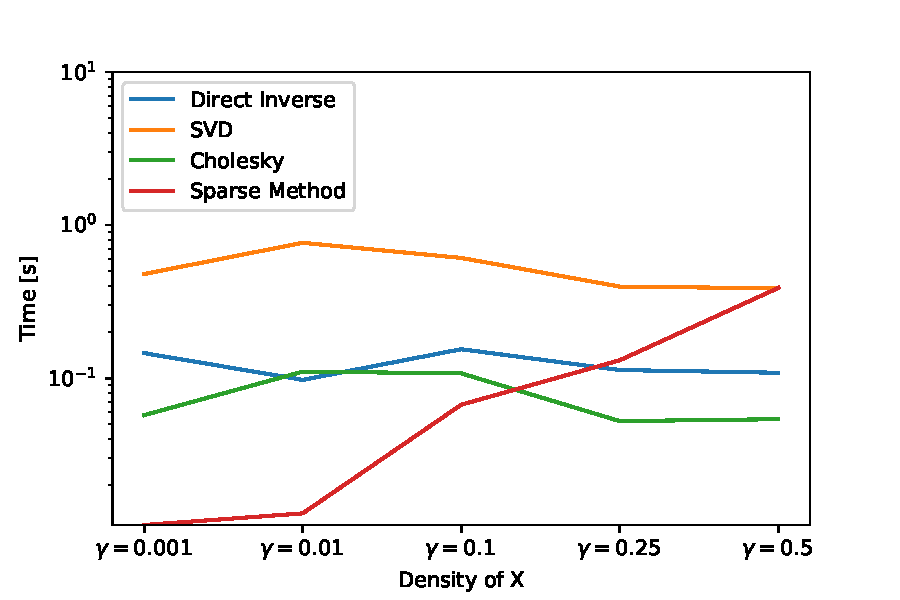
\includegraphics[width = \textwidth]{fig1}
\end{figure}

We can see that:
\begin{itemize}
	\item Method 1--3 do not exploit sparsity. Their CPU times do not change with density.
	\item When density is relatively small, the sparse method has an advantage over all the other three method. When density is relatively large, the sparse method is slower than Method 1 and 3, possibly due to overhead of the sparse data structure.
\end{itemize} 

\section{Generalized Linear Models}

\subsection{(A)}
We have $y_i \sim \text{Binomial}(m_i, w_i)$\footnote{For the simpler case of binary logistic regression where we have $y_i \sim \text{Bernoulli}(w_i)$, just apply $m_i = 1$ in the following results.}, where 
$$
		w_i = \frac{1}{1+\exp(-x_i^T\beta)},
$$
$$
1-w_i = \frac{\exp(-x_i^T\beta)}{1+\exp(-x_i^T\beta)}.
$$

The negative log likelihood function is:
\begin{align}
		\ell(\beta) &= -\log \left \{ \prod_{i=1}^N p(y_i | \beta)  \right \} \\
		&= -\log \left \{ \prod_{i=1}^N \binom {m_i}{y_i}(w_i)^{y_i}(1-w_i)^{m_i-y_i}  \right \} \\
		&= - \left \{ \sum_{i=1}^{N} \left ( \log\binom {m_i}{y_i} + y_i \log(w_i) + (m_i-y_i)\log(1-w_i) \right ) \right \} 
	\end{align}
	
We have:
\begin{align}
\nabla \log w_i& = - \nabla \log (1 + \exp(-x_i^T\beta)	)\\
&= \frac{x_i \exp(-x_i^T\beta)}{1 + \exp(-x_i^T\beta)}\\
& = x_i(1-w_i)
\end{align}

\begin{align}
\nabla \log (1-w_i) & = \nabla (-x_i^T\beta)- \nabla \log (1 + \exp(-x_i^T\beta)	)\\
&= -x_i + x_i (1 - w_i)\\
& = -x_iw_i
\end{align}



Therefore, the gradient of the loss function is:
\begin{align}
		\nabla \ell (\beta) &=\sum_{i=1}^N \left ( y_i x_i (1-w_i) - (m_i - y_i) x_i w_i \right ) \\
		&= \sum_{i=1}^N (m_iw_i-y_i)x_i \\
		&= X^T(m\circ w-y),
	\end{align}
where operator $\circ$ denotes element-wise product.

\subsection{(B)}

We use the data “wdbc.csv” from course website. We use the first 10 features in our model. We add a column of ones into $X$ matrix to represent the intercept term.

To alleviate the numerical issue brought by having a very large $w_i$ value, we first scale the $X$ data using \texttt{scikit-learn preprocessor}. 

We perform a naive gradient descent with different step lengths:
 \begin{itemize}
 	\item fixed step size of $0.001$,
 	\item fixed step size of $0.005$,
 	\item fixed step size of $0.01$, and
 	\item variable step size of $1/k$ where $k$ is the iteration count.
 \end{itemize}

 To clearly see the difference between different step sizes, we compute $50$ iterations. The codes are shown in \texttt{logit.py} and the loss function value as a function of iteration count is shown below:

\begin{figure}[!h]
\caption{Loss function value as a function of iteration count}
\centering
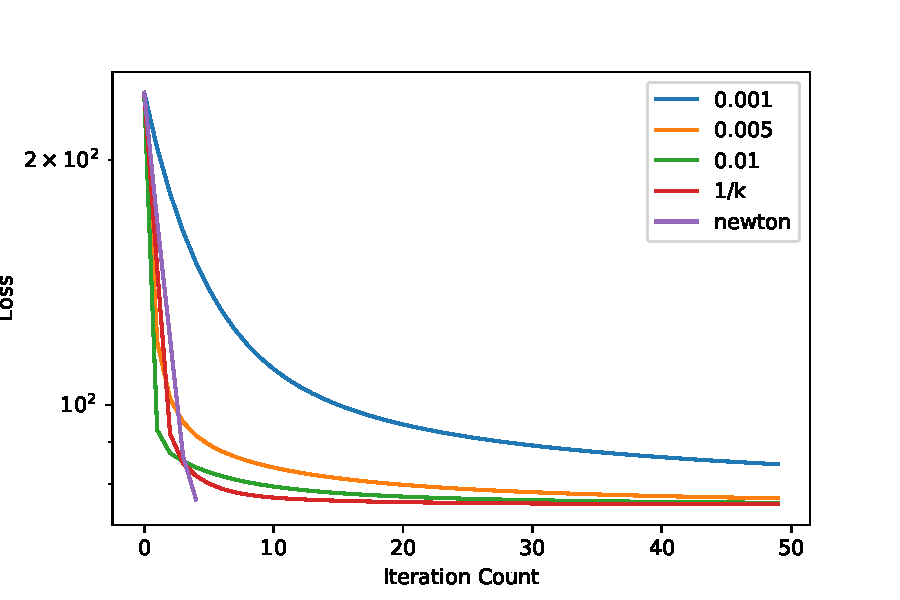
\includegraphics[width = \textwidth]{fig_logit}
\label{fig:results}
\end{figure}

The step size $0.01$ performs well for this dataset. For the first few iterations, the step sizes for the $1/k$ rule are too large, so that the loss function does not decrease as much.

I also implemented a \texttt{predict()} function that evaluates the training error of our logistic model. After only $50$ iterations, the training accuracy is $94.02\%$. 

\subsection{(C)}
Our objective is to compute the Taylor approximation:
$$
\hat{\ell}(\beta) = \ell(\beta_0)+(\nabla \ell(\beta))^T(\beta-\beta_0) + \frac{1}{2}(\beta-\beta_0)^T \nabla^2 \ell(\beta) (\beta-\beta_0).
$$
We have computed $\nabla \ell(\beta)$ in section (A). Now we compute the $(i,j)$ element of the Hessian $\nabla^2 \ell(\beta)$:
\begin{align}
		\frac{\partial^2}{\partial \beta_i \partial \beta _j}\ell (\beta) 
		&= \frac{\partial}{\partial \beta_i} \left ( \nabla_j \ell(\beta) \right ) \\
		&= \frac{\partial}{\partial \beta_i} \left ( \sum_{k=1}^N(m_kw_k-y_k)x_{kj} \right )  \\
		&= \sum_{k=1}^{N} x_{ki}x_{kj}m_k w_k(1-w_k),
	\end{align}
where we use the fact that 
$$
		\frac{\partial}{\partial \beta_i} w_k = x_{ki} w_k(1-w_k).
$$
We can define a new diagonal matrix $W = \text{diag}(m_1w_1(1-w_1),\ldots, m_Nw_N(1-w_N))$, then we can write the Hessian in matrix form:
$$
\nabla^2 \ell(\beta) = X^TWX.
$$

Plugging in the expressions of the gradient and Hessian into the Taylor approximation yields:
$$
\hat{\ell}(\beta) = \ell(\beta_0) + (X^T(m\circ w-y))^T(\beta - \beta_0) + \frac{1}{2}(\beta - \beta_0)^T X^T W X (\beta - \beta_0).
		$$
		
Since we do not care about the constant term, we do not keep track of it in the following derivation. Instead, we use $c$ to represent the constant term, without specifying what $c$ is. Using the technique from: \url{https://justindomke.wordpress.com/completing-the-square-in-n-dimensions/}, we can continue our reformation:
\small
\begin{align*}
		\hat{\ell}(\beta) 
		&= \frac{1}{2} ( [ \beta - \beta_0 ] +(X^T W X)^{-1} X^T (m\circ w-y) )^T X^T W X ( [ \beta - \beta_0 ] +\\
		& \quad \quad (X^T W X)^{-1} X^T (m\circ w-y) ) + c' \\ 
		&= \frac{1}{2} (\beta - \beta_0 - X^{-1}W^{-1} (m\circ w-y) )^T X^T W X (\beta - \beta_0 - X^{-1}W^{-1} (m\circ w-y) ) + c' \\
		&= \frac{1}{2} (X\beta - X\beta_0 + W^{-1} (m\circ w-y) )^T W (X\beta - X\beta_0 + W^{-1} (m\circ w-y) ) + c'' \\
		&= \frac{1}{2}(z-X\beta)^T W (z-X\beta) + c,
	\end{align*}
where $z = X\beta_0 + W^{-1}(y-m\circ w)$.

\subsection{(D)}

Now we use Newton's method to perform our loss minimization. The update rule is as follows:
$$
	\hat{\beta}_{t+1} = \hat{\beta}_t - (\nabla^2\ell(\hat{\beta}_t))^{-1}\nabla\ell(\hat{\beta_t}),
$$
where we have computed the Hessian in the previous subsection.

The results of the Newton's method are also given in Fig. \ref{fig:results}. We can see that after four iterations, the gradient is already very close to zero ($< 10^{-14}$).

\subsection{(E)}

Reflections:
\begin{itemize}
	\item Gradient descent requires more iterations, and there is no simple way to determine which step size rule is better. 
	\item Newton's method converges with far fewer iterations because we are using second-order information. 
	\item For Newton's method, we need to compute the Hessian matrix, and solve a linear system in each iteration. The computational effort per iteration is greater.
\end{itemize}






%\bibliographystyle{IEEEtran}
%\bibliography{gas}
\end{document}

